\subsection{Test 4: Monologue Tests}
This section looks at self recordings and recordings from others online. This was done to increase the variance through different voice types, recording types (freq?)?, different cadences, different recording environments. 

Pauses were counted for some, but more will be done.

\paragraph{Test 4.1:} Grab pauses for a self made audio file (e.g. not from the talk bank)

This is in ideal conditions where the bitrate is high, the pauses are distinct and clear

Remember to Get the pauses checked for correctness once I show I can get a histogram i.e. manually go through and see that pauses are accounted for to show the validity of the algorithm/code 

\paragraph{Test 4.2:} Grab speech audio file from online, test, grab histograms 

\paragraph{Test 4.2.1:} Open Speech Repository (Is this an experiment?)

Reason for Experiment: This was used to show a distinction between the natural conversations taken from E1.2.2 and the more stilted pausing of this recording. 

The downside to this was the pause distribution it produced is of a different conversation type, monologue instead of dialogue. And the audio files are only 30 seconds in length compared to the 30min avg for the talkbank files. So pause frequencies were not as abundant as they would be for longer files. I decided to take the collection of pause frequencies and plot them on a single histogram. I also plotted the change in pause types between male and female speakers. 

- URL to repo
https://www.voiptroubleshooter.com/open\_speech/american.html

Another way to do this would be to grab lectures and see how they compare. They would be much longer and give more detailed pause analysis and I'm sure there a bunch of good quality lecture recordings I could grab to do this on. 

/ca/SCOTUS/OralArguments/ was another that showed multiple single speakers

\subsubsection{Female speaker}
Reason for experiment: 
\paragraph{Test 4.2.1: Lady Speaking 1}
    
Audio file link, Raw pause output
Histogram figure: 

\begin{figure}[h]
    \centering
    \begin{minipage}{0.45\textwidth}
        \centering
        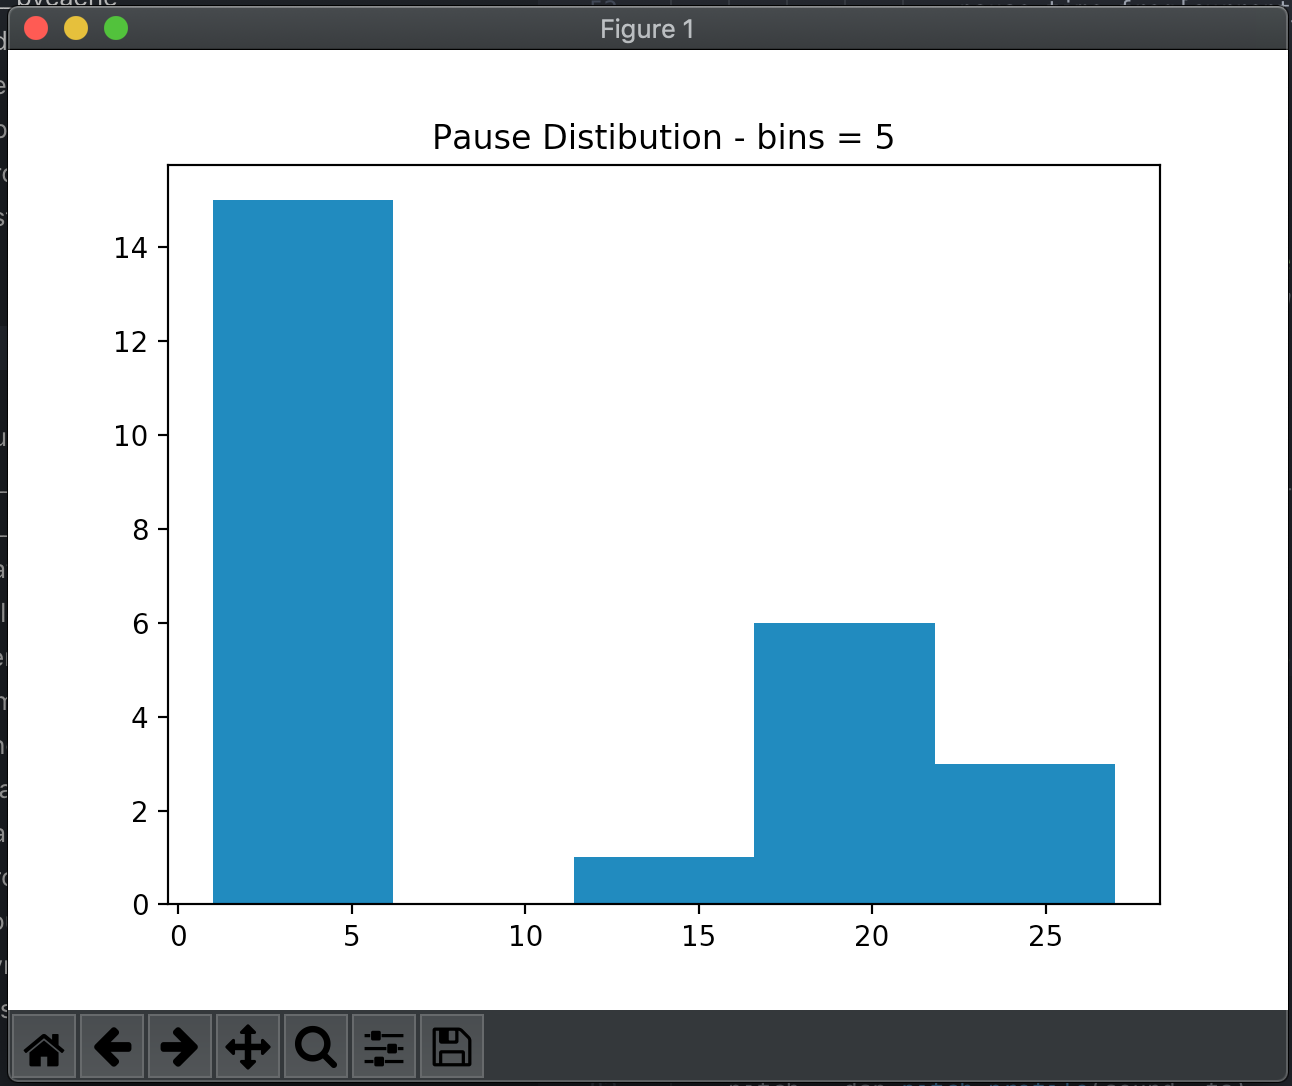
\includegraphics[scale=0.2]{src/main-matter/methodology/pause-distributions/monologue/lady1-1} 
        \caption{Lady Speaking 1-1}
    \end{minipage}\hfill
    \begin{minipage}{0.45\textwidth}
        \centering
        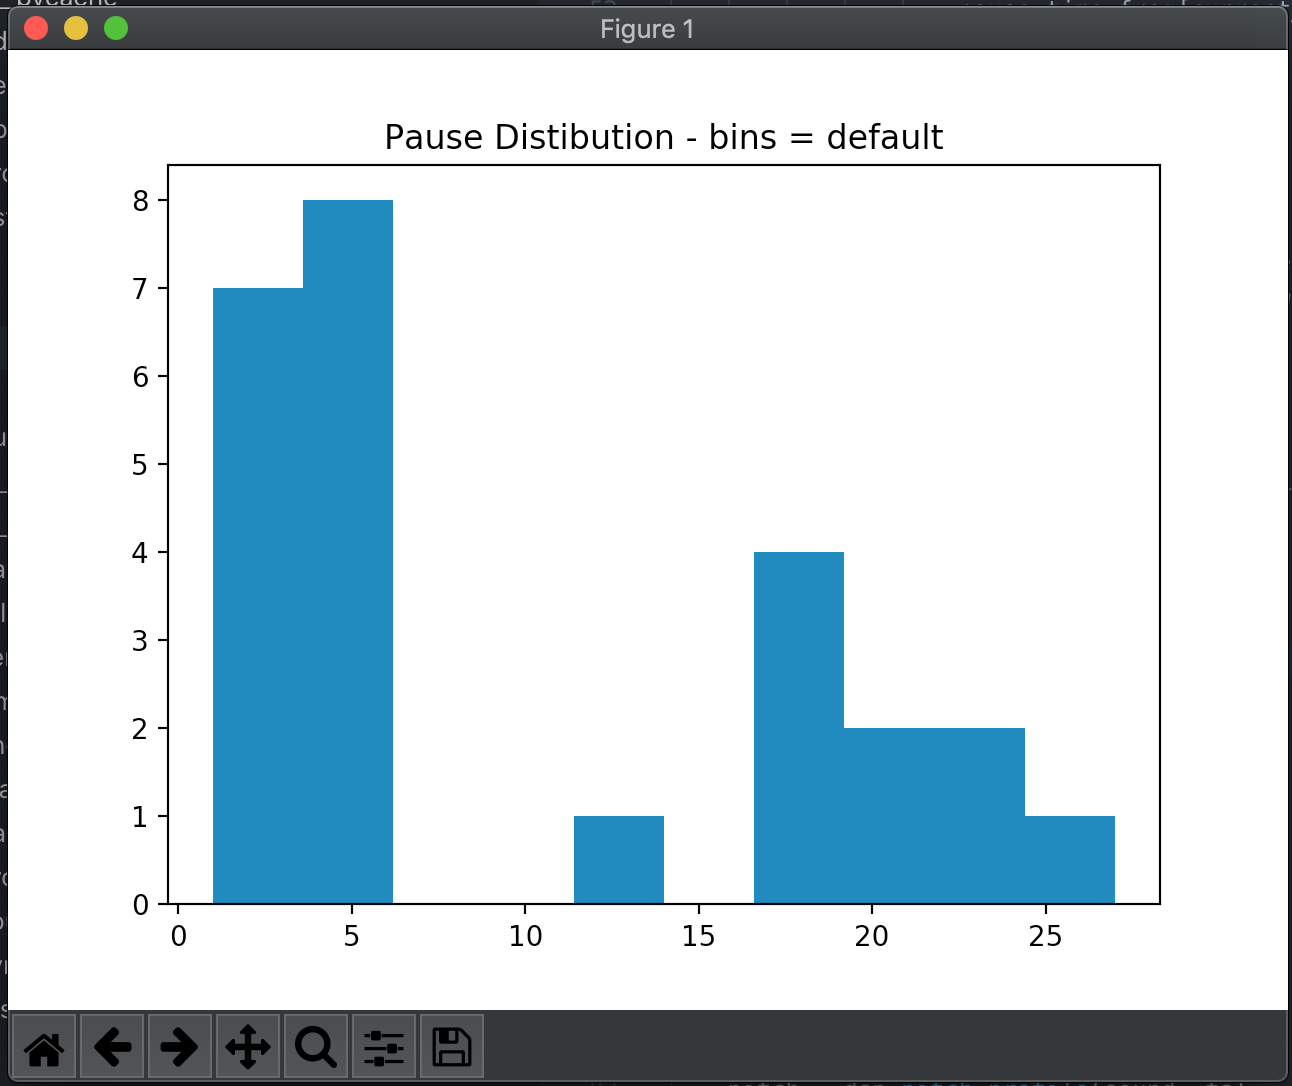
\includegraphics[scale=0.2]{src/main-matter/methodology/pause-distributions/monologue/lady1-2} 
        \caption{Lady Speaking 1-2}
    \end{minipage}\hfill
    \begin{minipage}{0.45\textwidth}
        \centering
        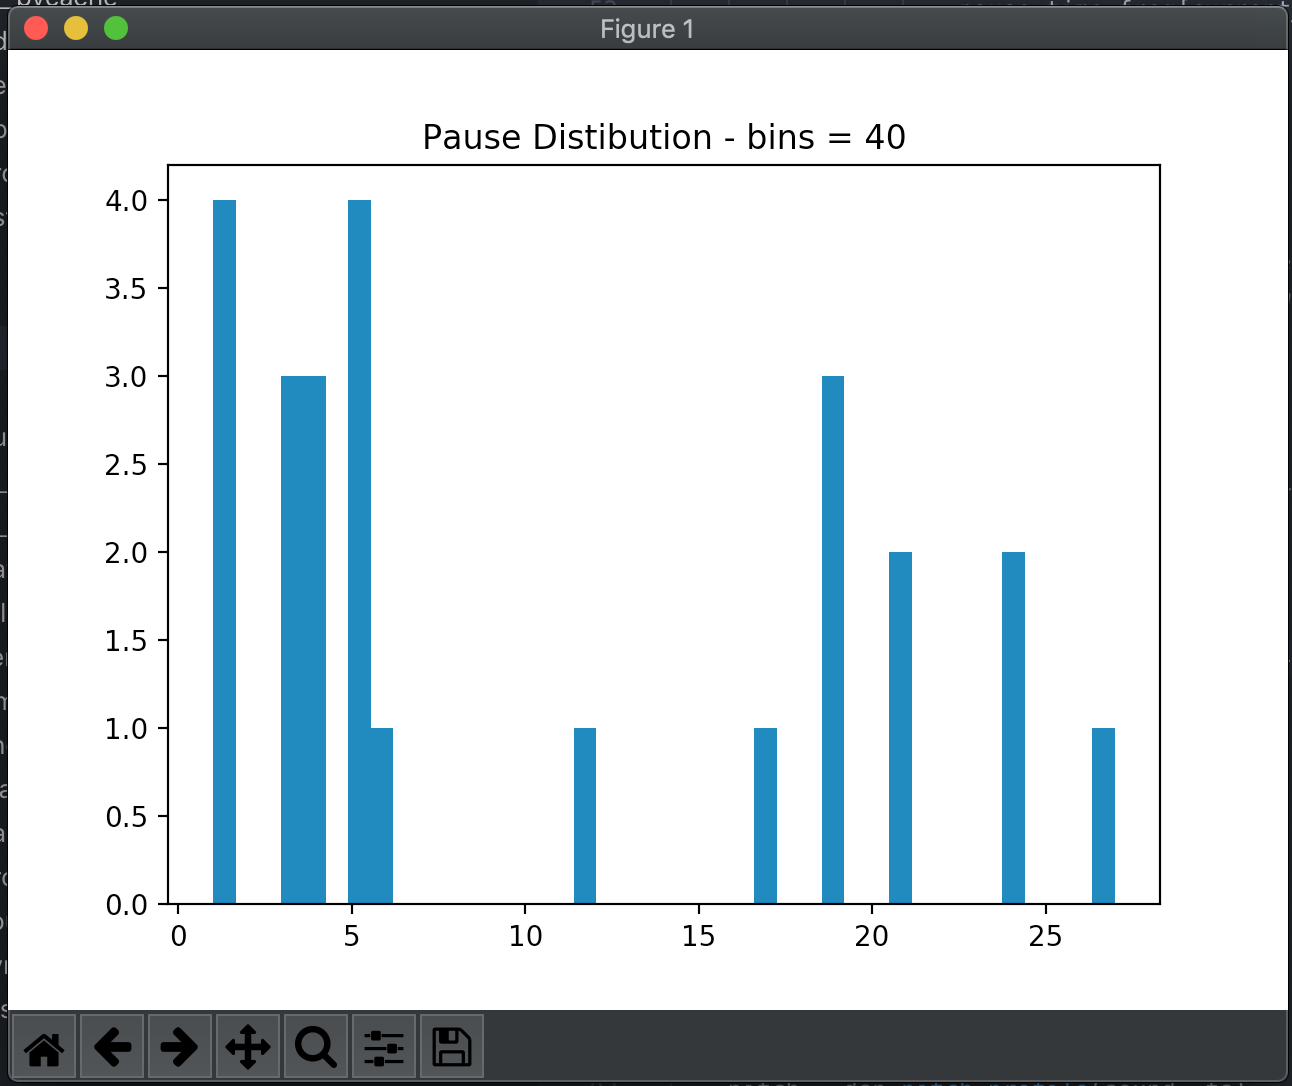
\includegraphics[scale=0.2]{src/main-matter/methodology/pause-distributions/monologue/lady1-3} 
        \caption{Lady Speaking 1-3}
    \end{minipage}
\end{figure}

Findings: Pauses tended to clump together around 0-20ms

\paragraph{Test 4.2.2: Lady Speaking 2}
Link to Audio file, Raw pause output

Histogram
Findings
        
        
        
\subsubsection{Male Speaker}
\paragraph{Test 4.2.3: Man Speaking - 1}
Audio file, Raw pause output can be found at the output\\monologue\\OSR\_us\_000\_0030\_8k directory
Histogram 
\begin{figure}[h]
	\begin{center}
		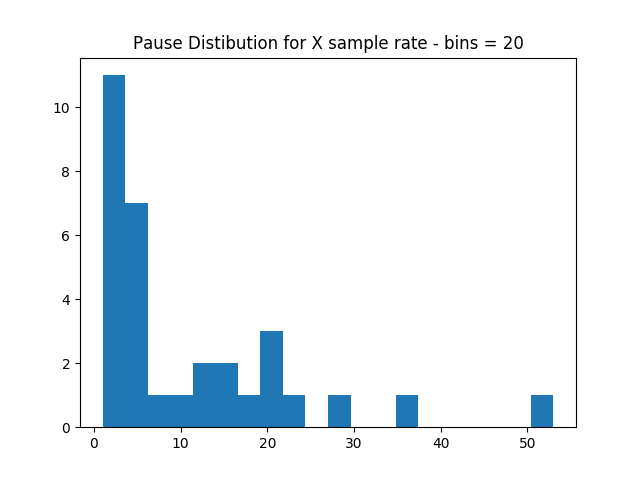
\includegraphics[scale=0.2]{src/main-matter/methodology/pause-distributions/monologue/man1-1}
		\caption{Man Speaking 1-1}
		\label{default}
	\end{center}
\end{figure}
Findings: Pauses tended to clump together around 0-20ms, Should test on wider bin size

\paragraph{Test 4.2.4: Man Speaking 2} 
Link to Audio File, pause output - (OSR\_us\_000\_0061\_8k)
list data output directory location that has everything we need in it
Histogram: 
Findings: Pauses tended to clump around 0-10ms, maybe smaller grained, Needed to test on wider bin 

\paragraph{Test 4.2.5: Man Speaking 3}
\begin{figure}[h]
	\begin{center}
		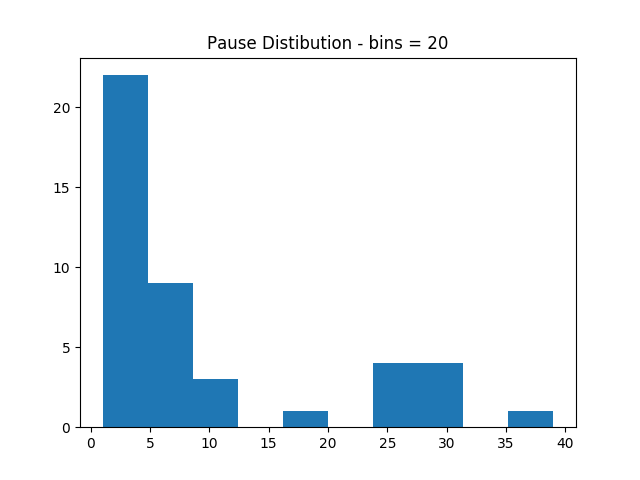
\includegraphics[scale=0.2]{src/main-matter/methodology/pause-distributions/monologue/man2-1}
		\caption{Man Speaking 2-1}
		\label{default}
	\end{center}
\end{figure}
    Findings


\paragraph{Conclusions:} These experiments showed a tendency, even in stilted audio, to tend towards short pauses around the 0-20ms mark. Where the curve tended to be heavily right skewed.